\documentclass[a4paper]{article}
\usepackage{pdfpages, pgffor}
\setlength{\fboxrule}{0.3mm}

\begin{document}
\newwrite\myoutput
\immediate\openout\myoutput=\jobname.options
\immediate\write\myoutput{\unexpanded{\documentclass[10pt, handout, aspectratio=169]{beamer}}} %43 for 4x3, 169 for 16x9, 1610 for 16x10
\immediate\closeout\myoutput
\foreach \n in {1,...,8}{
    \IfFileExists{week\n/week\n.tex}{
        \immediate\write18{texify.exe --pdf  --clean week\n/week\n.tex}
        \includepdf[pages=-,nup=2x2,delta=5pt 30pt,landscape=true,frame=true,column=false,noautoscale=false]{week\n.pdf}
    }
}
\end{document}

\usetheme{Frankfurt}
\usecolortheme{crane}

\usepackage{exscale,latexsym,microtype,amsmath,amssymb,amsfonts,graphicx,natbib,times,booktabs,xstring}

\newcommand{\E}{\ensuremath{{\mathbb E}}} % expected value
\newcommand{\R}{\ensuremath{{\mathbb R}}}
\newcommand{\Var}{\ensuremath{{\mathbb V}}} % variance
\newcommand{\frameit}[2]{\begin{frame}\frametitle{#1}\begin{itemize}#2\end{itemize}\end{frame}}
\def\func#1{\mathop{\rm #1}}
\def\er#1{\emph{\color{red}#1}}
\def\newblock{\hskip .11em plus .33em minus .07em}
\def\limfunc#1{\mathop{\rm #1}}%
\setbeamertemplate{blocks}[rounded][shadow=true]
\date{}

\titlegraphic{
\includegraphics[height =0.4in]{../HSLU_Logo_EN_Schwarz_rgb}}
\title{Module 9.3: Time Series Analysis with Python\\Fall Term\space\number\year}
\def\theweek{\StrRight{\jobname}{1}}
\author[Week \theweek]{\textbf{Week \theweek}:}
\AtBeginSection{
\frame{
\frametitle{Outline}
\tableofcontents[currentsection]
}}


\institute{{\Large Unit Roots; ARIMA Models}}
\begin{document}
\frame{\titlepage}
\begin{frame}%
\frametitle{Outline in Weeks}
\begin{enumerate}
\item Introduction; Descriptive Modeling
\item Returns; Autocorrelation; Stationarity
\item ARMA Models
\item Unit Roots; ARIMA Models
\item Volatility Modeling
\item Value at Risk
\item Cointegration
%\item Panel Data
\end{enumerate}
\end{frame}% 

\section{Unit Root Testing}\subsection*{bla}
\begin{frame}{Unit Root Testing}
\begin{itemize}
\item Recall that if a nonstationary series, $y_t$ must be differenced
$d$ times before it becomes stationary, then it is said to be \emph{\color{red}integrated} of order $d$. Notation: I$(d)$. When we simply say
`integrated' we mean I$(1)$. Another synonym is `the series has a \er{unit root}'.

\item So far, our decision to take differences was
based on the correlogram: if autocorrelations decay
slowly and approximately linearly, then the series may be integrated and must
be differenced.

\item This procedure is subjective and unreliable:
 a \er{trend-stationary} series, such as $Y_{t}=\beta_0 +\beta_1 t+U_{t}$%
, will also have large and slowly decaying autocorrelations (see \texttt{simulation.xlsx}).

\item  Therefore, it
is useful to have a formal testing procedure to distinguish integrated from
(trend-) stationary time series. Such tests are called \emph{\color{red}unit root
tests}. The \er{(Augmented) Dickey-Fuller} test is the most common.


\end{itemize}
\end{frame}
\begin{frame}
\frametitle{Example: the AR(1) Model}

\begin{itemize}
\item The simplest example of stationary and integrated time series is
the AR(1) model
\begin{equation*}
Y_{t}=\phi_1 Y_{t-1}+U_{t},
\end{equation*}%
where $Y_0$ is a constant.

\item If $-1<\phi_1 <1$, then $Y_{t}$ is stationary, with mean $0$ and
variance $\sigma ^{2}/(1-\phi ^{2})$.

\item If $\phi_1 =1$, then the model becomes a \emph{\color{red}random walk}, $%
Y_{t}=Y_{t-1}+U_{t}$, with mean $Y_{0}$ and variance $\sigma ^{2}t$.
\end{itemize}
\end{frame}
\begin{frame}%
\frametitle{Stochastic vs. Deterministic Trends}

\begin{itemize}
\item Consider the two models
\begin{align*}
Y_{1,t}&=\delta t+U_{1,t} \quad\mbox{and}\\
Y_{2,t}&=\delta + Y_{2,t-1}+U_{2,t}.
\end{align*}
\item For both models, $\mathbb \E[\Delta Y_t]=\delta$, i.e., both series trend upwards by $\delta$ each period.
\item $Y_{1,t}$ contains a \emph{\color{red}deterministic trend}: $Y_{1,t}-\delta t=U_{1,t}$ is stationary. In practice, regress $y_t$ on a linear trend like in week 1; the residuals will be stationary.
\item $Y_{2,t}$ contains a \emph{\color{red}stochastic trend}: $Y_{2,t}-\delta t$ is a random walk. It becomes stationary only by differencing, i.e., it is $I(1).$
\end{itemize}

\end{frame}

\begin{frame}
\begin{block}{Random walk (left) vs.\ trend stationary process (right).}
\begin{tabular}{cc}
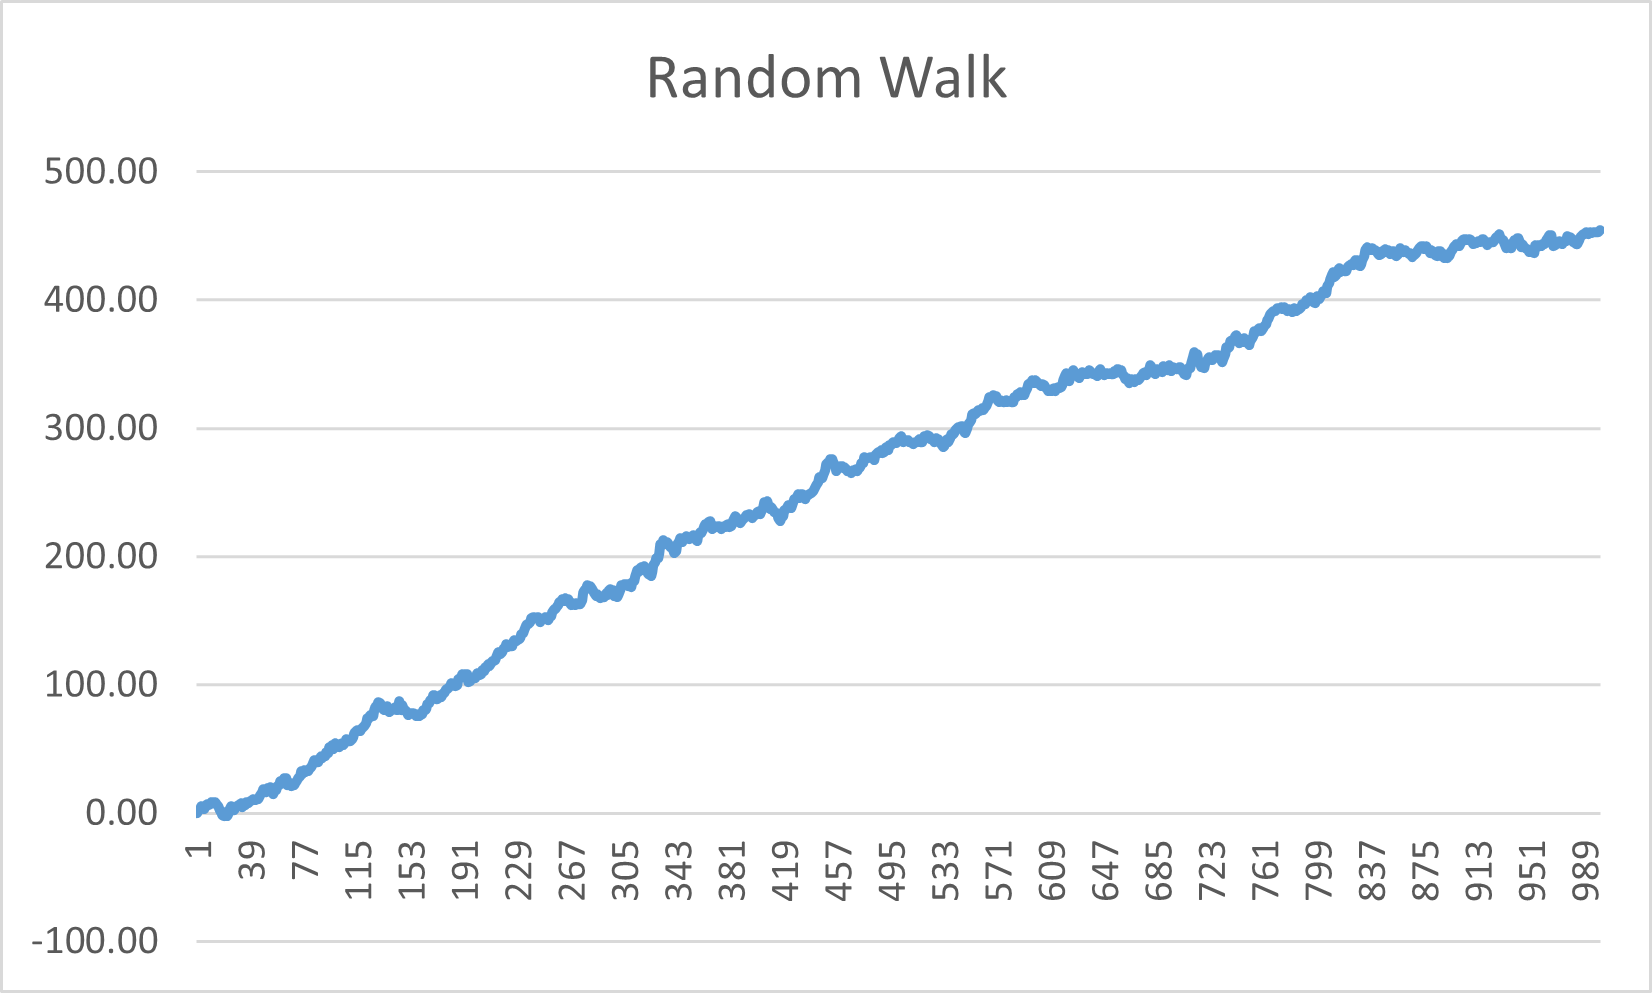
\includegraphics[width=0.4\textwidth]{rw1} & 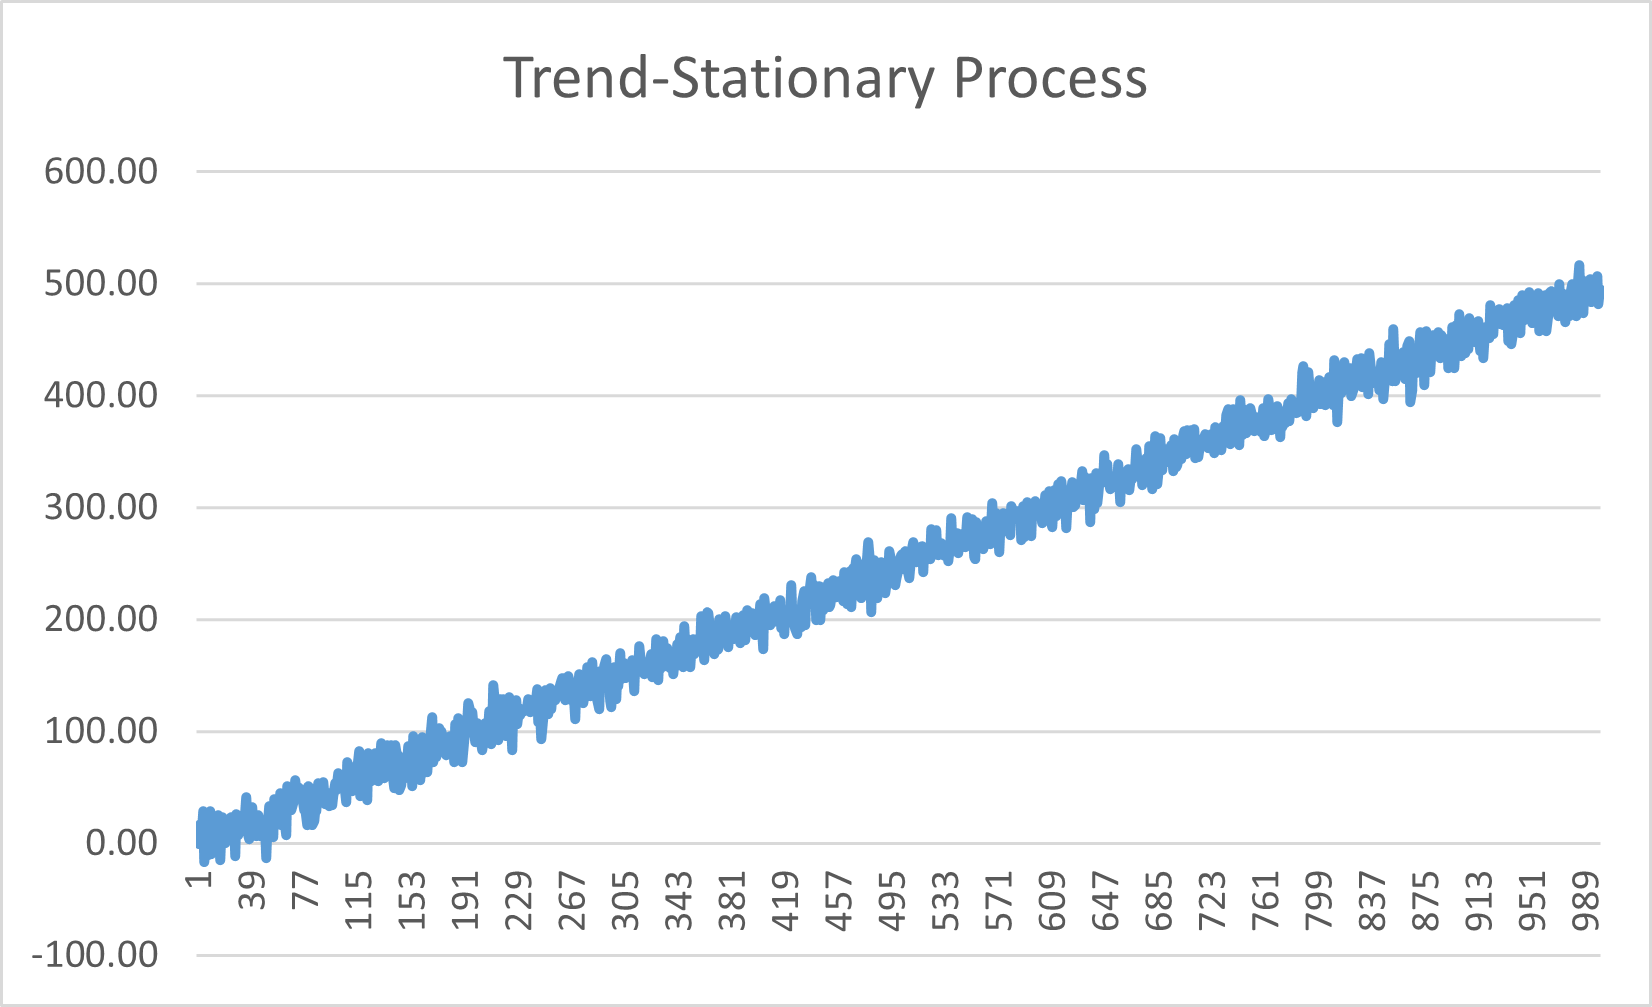
\includegraphics[width=0.4\textwidth]{ts1}\\
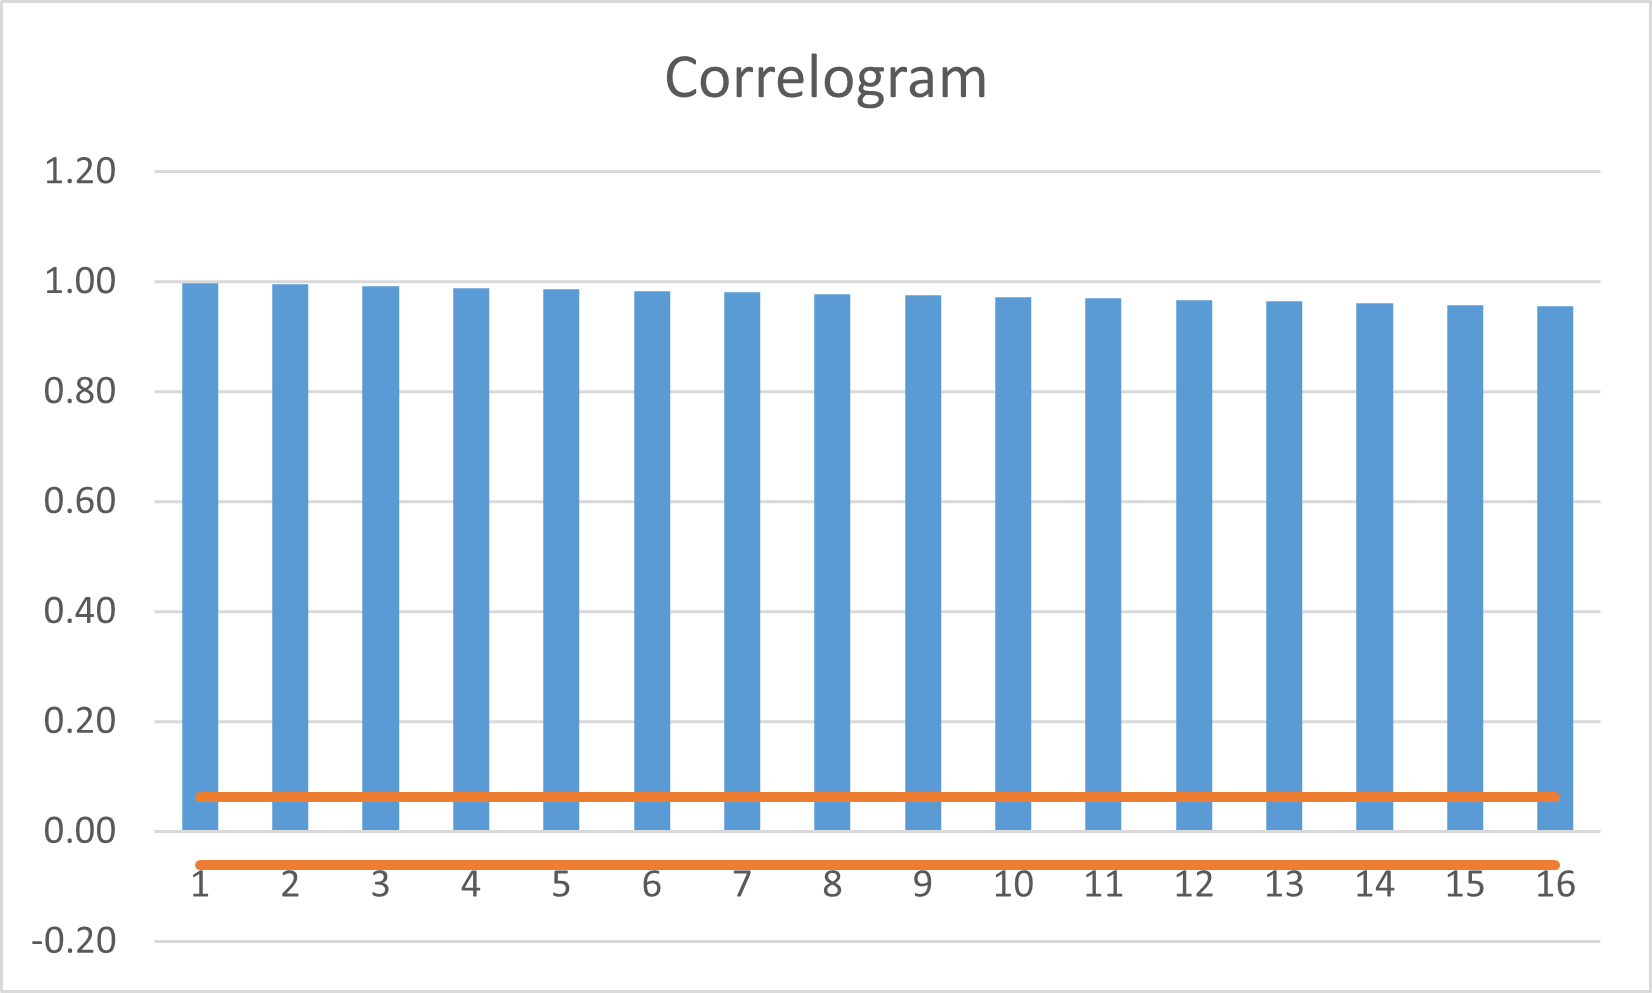
\includegraphics[width=0.4\textwidth]{rw2} & 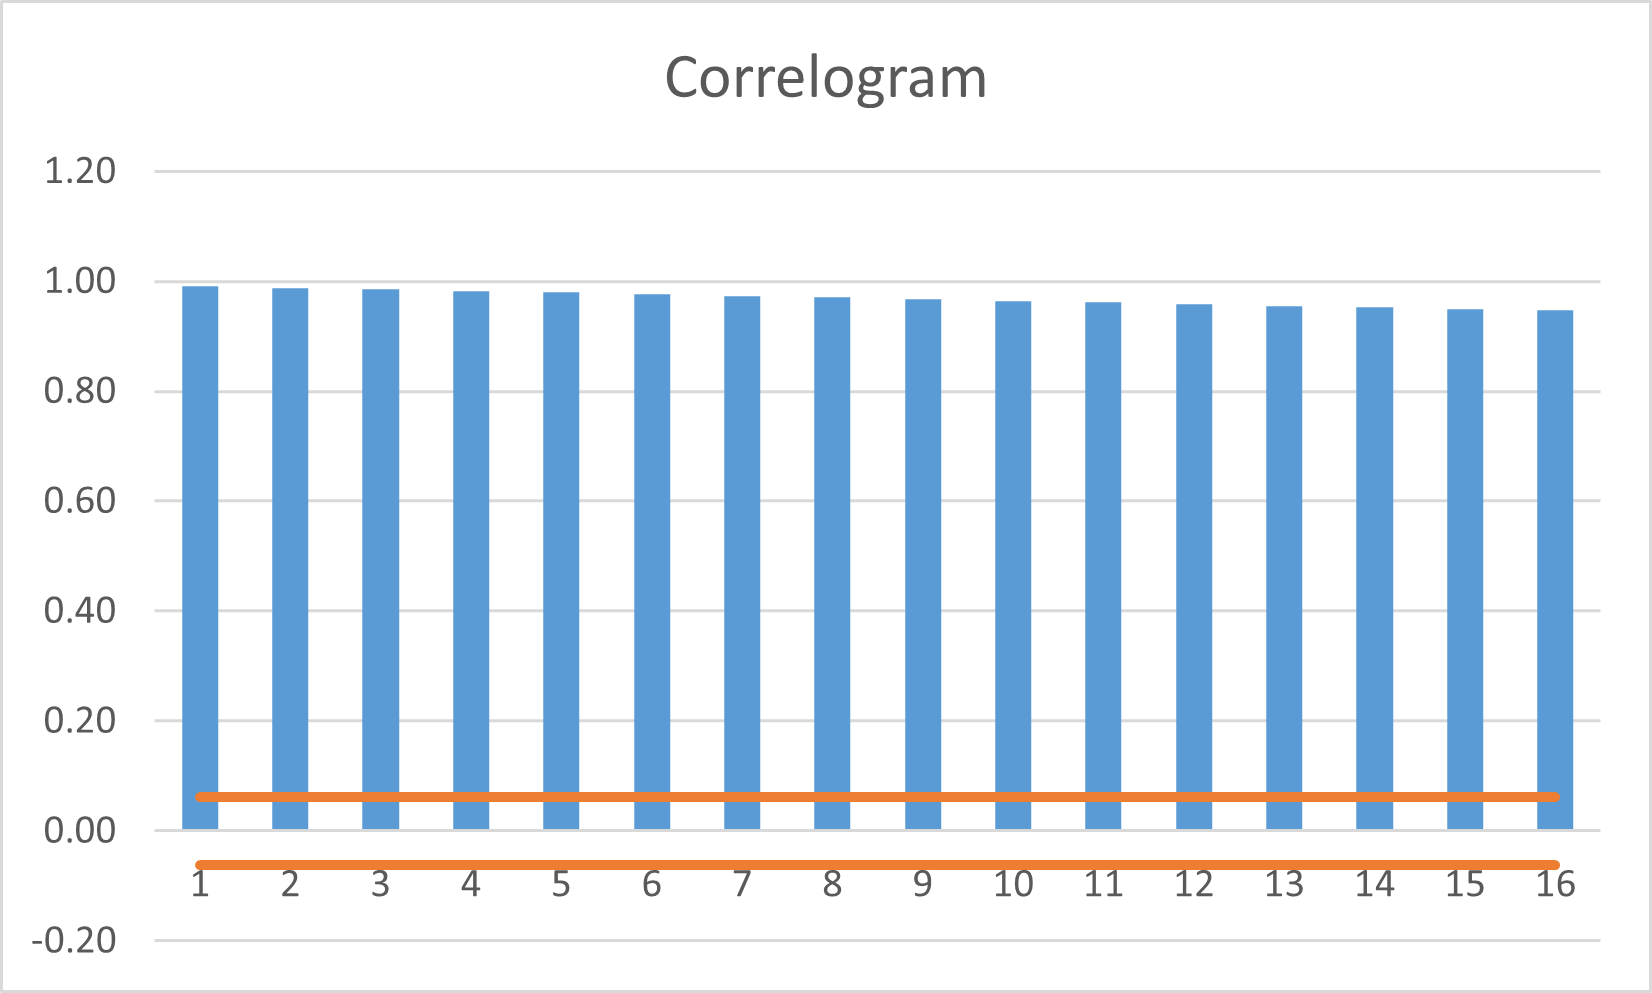
\includegraphics[width=0.4\textwidth]{ts2}
\end{tabular}
\end{block}
\end{frame}

\begin{frame}
\frametitle{Why do we care?}
\begin{enumerate}
\item Inference: OLS estimators have non-standard distribution, so that standard inference is invalid.
\item Forecasting:
\begin{itemize}
\item stationary series display \emph{\color{red}mean-reversion}; deviations from
the mean are corrected in the next period. Shocks $U_{t}$ have a \emph{\color{red}transitory}, decreasing effect
on future $Y_{t+k}$ (in AR(1) model, the effect is $\phi ^{k}\rightarrow 0$);
\item For integrated time series (of order 1): no mean-reversion, shocks $U_{t}$ have a \emph{\color{red}persistent} effect on future $Y_{t+k}$.
\end{itemize}
\item Spurious regression: regressing two drifting I(1) variables onto each other will spuriously result in significant estimates, because they happen to trend in the same direction.
\end{enumerate}
\end{frame}



\begin{frame}{The Dickey-Fuller Test}
\begin{itemize}
\item Consider again the AR(1) model
\begin{equation*}
Y_t = \phi_1 Y_{t-1} + U_t .
\end{equation*}
\item We wish to test the null hypothesis
$
H_0: \phi_1 = 1 ,
$
against the \emph{\color{red}one-sided} alternative hypothesis
$
H_1: \phi_1 <1 .
$

\item Under the null, the process is a random walk, and hence
integrated. Under the alternative, it is stationary (if $\phi_1 >-1$,
which we assume). Therefore, we will be testing $H_{0}:Y_{t}\sim
I(1)$ against $H_{1}:Y_{t}\sim I(0)$.

\item  The \er{Dickey-Fuller test} is
based on the $t$-statistic for $\phi_1 =1$ in the AR(1) model, which may be
reformulated as the $t$-statistic for $\psi =0$ in
\begin{equation*}
\Delta y_{t}=\psi y_{t-1}+u_{t},
\end{equation*}%
where $\psi :=\phi_1 -1$; note that $\psi <0$ under the alternative.

\end{itemize}
\end{frame}
\begin{frame}{The Dickey-Fuller Distribution}
\begin{itemize}
\item  We reject $H_{0}$ if the $t$-statistic is less than the
(negative) critical value.

\item In classical regressions, the $5\%$ critical value for a one-sided $t$-test
would be $-1.645$. However, because the regressor $Y_{t-1}$ is
non-stationary under the null, a different distribution arises,
and the appropriate $5\%$ critical value is $= -1.95$.

\item This critical value changes to $= -2.86$ if we add a
constant term to the regression:
\begin{equation*}
\Delta y_t = \alpha+ \psi y_{t-1}   + u_t.
\end{equation*}
This is the relevant
test if we want to allow for a non-zero mean $\E[Y_t]$ under the
alternative.

\item  If we want to test a random walk \emph{\color{red}with
drift} against a \emph{\color{red}trend-stationary} alternative, then the
relevant regression is
\begin{equation*}
\Delta y_t = \alpha+\delta t+\psi y_{t-1}  + u_t,
\end{equation*}
and the $5\%$ critical value is $= -3.41$.
\end{itemize}
\end{frame}
\begin{frame}{Choice of Model}
\begin{itemize}
\item The difference between the three tests is whether or not a constant and a time trend are included in the test regression.
\item In practice, the test without constant and trend  is
almost never applicable.

\item The test with an intercept in the regression test is relevant for series such
as interest
rates and real exchange rates, where we do not expect a linear trend under
either the null or the alternative hypothesis.

\item Many other economic and
financial time series, such as GDP or (log-)
asset prices, clearly display an upward trend, in which case a trend should be included.
\end{itemize}
\end{frame}

\begin{frame}{The Augmented Dickey-Fuller Test}
\begin{itemize}

\item The \emph{\color{red}augmented} Dickey-Fuller (ADF) test is an
extension of the procedure to the AR($p$) model
\begin{equation*}
Y_{t}= \phi _{1}Y_{t-1}+\ldots +\phi_{p}Y_{t-p}+ U_{t}.
\end{equation*}%
\item This process is integrated under $H_0: \phi_1 + \ldots + \phi_p = 1$, and
stationary under the alternative hypothesis $H_1: \phi_1 + \ldots + \phi_p <
1$.

\item It can be shown (see exercises) that this is equivalent to testing $H_0: \psi = 0$ against $%
H_1: \psi<0$ in the regression
\begin{equation*}
\Delta y_{t}= \psi y_{t-1}+\alpha _{1} \Delta y_{t-1}+\ldots +\alpha _{p^*}
\Delta y_{t-{p^*}}+ u _{t},
\end{equation*}
where $\psi =\sum_{i=1}^{p}\phi _{i}-1$, and $p^* = p-1$.

\item The interpretation of the null and alternative hypothesis, the role of the
constant and trend, and the critical values are the same as in the
first-order model.
\end{itemize}
\end{frame}
\begin{frame}
\frametitle{Choosing $p$}
\begin{itemize}
\item In practice,  $p$ is, of course, \er{unknown}.
\item The number of lags in the test regression must be chosen large enough, such that the residuals
have no autocorrelation, but not too large, because this would
decrease test power.
\item Often the choice is made based on \er{model selection criteria} (AIC, BIC). The \texttt{statsmodels} package has a built-in option to
do this automatically.
\item The AIC is preferred in this case, because it tends to include more lags than the BIC. This is preferred because our goal in this case is not to find the ``correct'' model, but to combat autocorrelation in the test regression.
\item So effectively, the ADF test is just the DF test (regress $\Delta y_t$ on $y_{t-1}$), but with enough lags of $\Delta Y_t$ thrown in to remove any autocorrelation.
\end{itemize}
\end{frame}
\section{ARIMA Models}\subsection*{bla}
\frameit{ARIMA Models}{
\item As discussed last week, the first step in the Box-Jenkins procedure is to make sure that the data are stationary.
\item This is usually decided by the ADF test.
\item If the test doesn't reject, then one models the first difference $\Delta Y_t$ as an ARMA process.
\item The model for the levels $Y_t$ is then called an \er{ARIMA($p$,$d$,$q$)} model: the data are differenced $d$ times, and the result modeled as an ARMA($p$,$q$) process. Usually, $d=1$.
\item To forecast an ARIMA process (with $d$=1), first predict $\Delta Y_{t+1}$, and then let $\hat{Y}_{t+1}=Y_t+\widehat{\Delta Y_{t+1}}$.
\item Longer horizon forecast are obtained recursively as usual.
}
%\section{Regressions with Time Series}\subsection*{bla}
%\begin{frame}%
%%EndExpansion
%\frametitle{Regression with Time Series}
%
%Some considerations when analyzing the relation between the time series $\{y_{t}\}$
%and $\{x_{t}\}$ in the regression model%
%\begin{equation*}
%y_{t}=\alpha +\beta' x_{t}+u_{t}:
%\end{equation*}
%
%\begin{itemize}
%\item Model is only reasonable if $Y_{t}$ and $X_{t}$ are integrated of same
%order. If both are $I(1)$, then in general the error will be $I(1)$, except
%in case of \emph{\color{red}cointegration} (stationary linear combination of $I(1)$
%series).
%
%\item In case of non-cointegrated $I(1)$ series, consider regression in
%first differences: $\Delta y_{t}=\alpha +\beta \Delta x_{t}+e_{t}$.
%
%\item Even when non-stationary is not a concern, autocorrelation usually is (most economic/financial series are autocorrelated).
%\item We will discuss two tests for autocorrelation in a regression: the \er{Breusch-Godfrey} test and the \er{Durbin-Watson} test.
%%\item Least-squares estimation is only consistent if $X_{t}$ is \emph{\color{red}
%%strictly exogenous} ($X_{t}$ independent of $U_{s}$ for all $t$ and $s$) or
%%\emph{\color{red}predetermined} ($\func{Cov}(X_{t},U_{s})=0$ for $t\leq s$).
%%
%%\item Neglected autocorrelation in errors $\{u_{t}\}$ can lead to violation
%%of predeterminedness. For example, if $X_{t}$ depends on $y_{t-1}$ and $%
%%U_{t}=\phi _{1}U_{t-1}+E_{t}$ with $\func{Cov}(X_{t},E_{t})=0$, then $\func{%
%%Cov}(X_{t},U_{t})\neq 0$.
%\end{itemize}
%\end{frame}%
%
%
%\begin{frame}
%\frametitle{Breusch-Godfrey Test}
%
%\begin{itemize}
%
%\item The \er{Breusch-Godfrey LM test} is done in four steps:
%
%
%\begin{enumerate}
%\item Estimate the regression, e.g.,%
%\begin{equation*}
%y_{t}=\beta _{1}+\beta _{2}x_{2t}+\beta _{3}x_{3t}+u_{t},
%\end{equation*}%
%by OLS, and get the residuals $\widehat{u}_{t}$.
%
%\item Estimate the auxiliary regression%
%\begin{equation*}
%\widehat{u}_{t}=\gamma _{1}+\gamma _{2}x_{2t}+\gamma _{3}x_{3t}+\tau _{1}%
%\widehat{u}_{t-1}+\ldots +\tau _{r}\widehat{u}_{t-r}+v_{t}.
%\end{equation*}%
%Denote by $R_{aux}^{2}$ the $R^{2}$ of this regression.
%
%
%\item Test the null hypothesis of \emph{\color{red}no residual
%autocorrelation}%
%\begin{equation*}
%H_{0}:\tau _{1}=\ldots =\tau _{r}=0,
%\end{equation*}%
%by the usual F-test, or by the LM test:%
%\begin{equation*}
% T \cdot R_{aux}^{2}\sim \chi ^{2}\left( r\right)
%\end{equation*}
%
%\item The test rejects for large values of $T \cdot R_{aux}^{2}$.
%\end{enumerate}
%\end{itemize}
%\end{frame}
%\begin{frame}
%\frametitle{Remarks}
%\begin{itemize}
%
%\item How do we choose $r$? Consult the correlogram, and take account of the
%frequency of the data, e.g., $r=4$ or $5$ for quarterly data.
%
%\item This is a general autocorrelation test. It has power against any
%degree of possible autocorrelation.
%
%\item EViews: after estimation, click \texttt{View}$\rightarrow$ \texttt{Residual Diagnostics} $\rightarrow$ \texttt{Serial Correlation LM test}
%\end{itemize}
%\end{frame}
%
%
%\begin{frame}
%\frametitle{The Durbin-Watson Test}
%\begin{itemize}
%\item  The \er{Durbin Watson} test is a test of first-order autocorrelation only.
%\item This test is performed as follows:
%
%\begin{enumerate}
%\item Get the OLS residuals $\widehat{u}_{t}$ from the regression as before.
%
%
%\item Compute the statistic%
%\begin{equation*}
%DW=\frac{\sum_{t=2}^{n}\left( \widehat{u}_{t}-\widehat{u}_{t-1}\right) ^{2}}{%
%\sum_{t=2}^{n}\widehat{u}_{t}^{2}}\approx 2\left( 1-\widehat{\tau }\right) .
%\end{equation*}%
%where $\hat{\tau}$ is OLS estimator of regression of $\widehat{u}_{t}$ on $%
%\widehat{u}_{t-1}$. Since $-1 \leq \widehat{\tau }\leq 1$, it follows that $0\leq DW\leq 4.$
%If there is no autocorrelation, we expect $DW\approx 2$.
%
%\item Look up the critical values for the test in a table. The test has a non-standard distribution. There are five different
%regions that lead to different conclusions (see next slide).
%\end{enumerate}
%\item The DW test is included in EViews estimation output by default.
%\end{itemize}
%\end{frame}
%
%\begin{frame}
%\frametitle{Test Decision}
%\begin{itemize}
%\item The critical values depend on the regressors. However, one can obtain bounds on the critical values.
%\item  The table gives the DW lower ($d_l$) and upper ($d_u$) bounds, at the $5\%$ level, for different values of $n$ and $k$. Test decision:
%\[
%\begin{array}{rrrrrll}
%0&<&DW & < & d_l &\Rightarrow &\text{reject (positive AC)}\\
%d_l&< &DW & < & d_u &\Rightarrow &\text{inconclusive}\\
%d_u&< &DW & < & 4-d_u &\Rightarrow &\text{do not reject}\\
%4-d_u&< &DW & < & 4-d_l &\Rightarrow &\text{inconclusive}\\
%4-d_l&< &DW & < & 4 &\Rightarrow &\text{reject (negative AC)}
%\end{array}
%\]
%\end{itemize}
%\end{frame}
%
%\begin{frame}
%\begin{block}{Critical Values of the DW Test}
%\begin{center}
%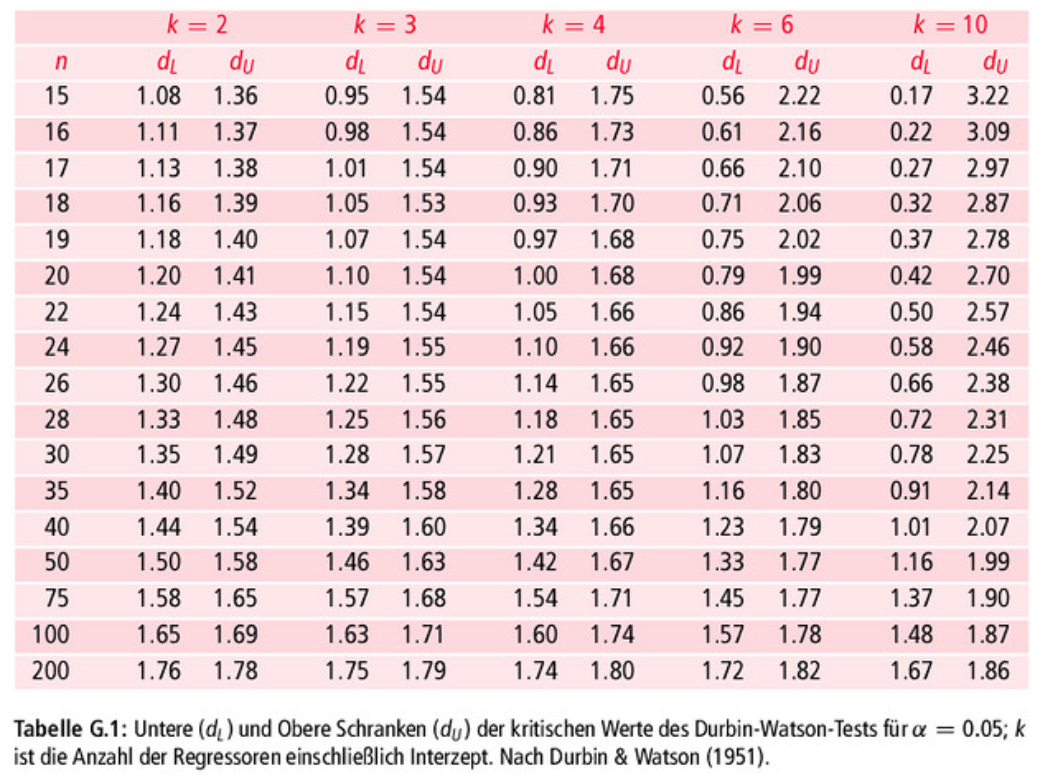
\includegraphics[width=.6\textwidth, trim=0 10ex 0 0, clip]{dwtable}
%\end{center}
%\small $\alpha=5$\%, $k=$ number of regressors (including intercept).
%\end{block}
%\end{frame}
%\begin{frame}
%\frametitle{Consequences of Autocorrelation}
%\begin{itemize}
%\item Only in a truly static model, the OLS estimator remains unbiased.
%
%\item In general, $\widehat{\beta}$ will be biased.
%
%\item OLS is no longer BLUE even when it is unbiased. More efficient estimators are available (GLS).
%
%\item The OLS standard errors are wrong.
%
%\item Inference based on usual $t$- and $F$-tests is unreliable.
%\end{itemize}
%\end{frame}
%\begin{frame}
%\frametitle{Solutions}
%\begin{itemize}
%
%\item One should at least use Newey-West \er{heteroskedasticity and autocorrelation consistent} (HAC) standard errors (in Eviews: Click on the \texttt{Options} tab when entering the regression equation)\footnote{EViews also provides \emph{\color{red}White standard errors}. These are consistent under heteroskedasticity only, not under autocorrelation.}.
%\item The more modern approach is to model the autocorrelation explicitly, by including lags of $y_t$ ($\rightarrow$ \er{ARX} model) and possibly $x_t$ ($\rightarrow$ \er{ADL}\footnote{autoregressive distributed lag} model). MA terms can also be added ($\rightarrow$\emph{\color{red}ARMAX} model).
%\end{itemize}
%\end{frame}
%
%%EndExpansion
%
%\begin{frame}
%\frametitle{Example}
%\begin{itemize}
%\item
%Consider the ADL model%
%\begin{equation}
%Y_{t}=\alpha_{0}+\alpha_{1}Y_{t-1}+\beta_{0}X_{t}+\beta_{1}X_{t-1}+u_{t}.
%\label{eq: ADL(1,1)}
%\end{equation}
%
%\item The \er{long-run equilibrium} is the \emph{\color{red}steady state} of the system $\left( Y_{t},X_{t}\right) $ when all
%future shocks $U_{t+1},U_{t+2},...$ are set to zero. If the system is
%stationary, then
%\begin{equation*}
%Y_{t}\rightarrow Y^{\ast }\text{ \ and \ }X_{t}\rightarrow X^{\ast }.
%\end{equation*}%
%So the long-run equilibrium can be found from the equation%
%\begin{align}
%Y^{\ast }& =\alpha _{0}+\alpha _{1}Y^{\ast }+\beta _{0}X^{\ast }+\beta
%_{1}X^{\ast }\Rightarrow  \notag \\
%Y^{\ast }& =\frac{\alpha _{0}}{1-\alpha _{1}}+\frac{\beta _{0}+\beta _{1}}{%
%1-\alpha _{1}}X^{\ast }.  \label{eq: static lr solution}
%\end{align}
%\end{itemize}
%\end{frame}
%\begin{frame}
%\frametitle{Why is a dynamic model needed?}
%A dynamic model can be necessary for the following reasons:
%\begin{itemize}
%\item Inertia of the dependent variable. E.g., adjustment costs, habits in
%individual decisions, or market frictions.
%
%\item Trending behaviour. E.g., if returns are unpredictable, prices must be
%trending. Hence, prices are autocorrelated.
%
%\item Seasonality; see Lecture 1.
%
%\item Over-reactions. Typically the result of some market failure, but think
%of exchange rate overshooting.
%\end{itemize}
%\end{frame}
%
%\begin{frame}
%\frametitle{Residual Autocorrelation}
%\begin{itemize}
%\item Now assume that instead of the dynamic model \eqref{eq: ADL(1,1)}, the steady state equation \eqref{eq: static lr solution} is estimated:
%\[
%y_t=a_0+b_0 x_t+u_t
%\]
%\item This is known as \er{dynamic misspecification}. The effect of the lagged variables is then in the error term. Result: autocorrelated residuals.
%\item In this case, not only the standard errors will be wrong, but the estimates will be biased: $\hat{b}_0$ will be an estimate of $\frac{\beta _{0}+\beta _{1}}{1-\alpha _{1}}$ in \eqref{eq: static lr solution}, not of $\beta_0$ in \eqref{eq: ADL(1,1)}.
%\item The modern view is that autocorrelation is not a problem, but an \er{opportunity to improve the model}.
%\item Thus, instead of correcting the standard errors, one should estimate a dynamic model directly.
%\item Start with a dynamic model (include lags of $Y_{t}$ and $X_{t}$ in the
%model). Test for autocorrelation, and for the significance of dynamics.
%%\begin{equation*}
%%\limfunc{cov}\left( U_{t},U_{t-j}\right) \neq 0\text{, for some }j>0.
%%\end{equation*}%
%\end{itemize}
%\end{frame}
%
%%\begin{frame}
%%\frametitle{Solutions II}
%%\begin{itemize}
%%\item In the special case of AR(1) errors, an alternative to HAC  standard errors is the  \er{Cochrane-Orcutt procedure}, a form of feasible GLS: Assume
%%\begin{align}
%%Y_{t}& =\beta  x_{t}+u_{t} \label{corc1}\\
%%u_{t}& =\tau u_{t-1}+v_{t}\label{corc2}
%%\end{align}
%%\item This can be rewritten as
%%\begin{equation}
%%Y_{t}-\tau Y_{t-1}=\beta (x_{t}-\tau x_{t-1})+v_{t}\label{corc3}
%%\end{equation}%
%%\item Idea: errors in \eqref{corc3} are not autocorrelated!
%%\item Cochrane and Orcutt suggest estimating \eqref{corc1} first to get residuals $\hat{u}_t$, then \eqref{corc2} to get $\hat{\tau}$, then construct $Y_t^{\ast}=Y_{t}-\hat{\tau} Y_{t-1}$
%%and $x_t^{\ast}=x_{t}-\hat{\tau} x_{t-1}$, and then estimate \eqref{corc3}.
%%\item In Eviews: similar effect by including \texttt{AR(1)} as an additional regressor.
%%\end{itemize}
%%\end{frame}
%%\begin{frame}\frametitle{Example: Traffic Count Data}
%%\begin{center}
%%\includegraphics[width=0.8\textwidth]{traffic1}
%%\end{center}
%%DW OK, but only 1st order...
%%\end{frame}
%%
%%\begin{frame}\frametitle{Example: Breusch-Godfrey}
%%\begin{center}
%%\includegraphics[width=0.5\textwidth]{traffic2}
%%\end{center}
%%$u_{t-2}$ seems to be the culprit...
%%\end{frame}
%%\begin{frame}\frametitle{Example: Cochrane-Orcutt (ish)}
%%\begin{tabular}{cc}
%%\includegraphics[width=0.5\textwidth]{traffic3}&
%%\includegraphics[width=0.5\textwidth]{traffic4}\\
%%\includegraphics[width=0.5\textwidth]{traffic5}&
%%\end{tabular}
%%\end{frame}


\section{Epilogue}\subsection*{bla}
\begin{frame}\frametitle{Learning Goals}
Students
\begin{itemize}
\item understand the ADF test and can use it to test for unit roots,
\item are able to forecast ARIMA models,
\item understand the difference between static and dynamic models, and
\item know how to test for autocorrelation in a regression
\end{itemize}

\end{frame}

\frameit{Homework}{
\item Exercise 4
\item Questions 2 and 3 from Chapter 8 of Brooks (2019)
\item \er{Assignment 1}. Deadline: Sunday after next, 11.59 p.m.
}

\end{document}
